\section{Nonreciprocal behavior}
\label{sec:nonreciprocal_behavior}

From the experimental results of the previous section, an important aspect has been highlighted related to the nonreciprocal behavior of the structure when excited with a time-space modulated signal.
In this section we aim at further investigate this aspect by performing additional experimental tests on the structure.



\subsection{Tests description}
\label{subsec:nonreciprocal_behavior_setup}

Using the same geometry and setup as in the previous sections (see Section \ref{subsec:experimental_setup}), we aim at exciting the structure at the two directional band-gaps frequencies observed in the previous section when modulating the shunts at $f_m = \pm 2 kHz$ are be analyzed.

For convenience, we report in Figure \ref{fig:nonreciprocal_behavior_2kHz} a zoomed-in version of the dispersion diagram around the two directional band-gaps frequencies $f_{BG}^- = [10 11] kHz$ and $f_{BG}^+ = [8 9] kHz$.

\begin{figure}[H]
    \centering
    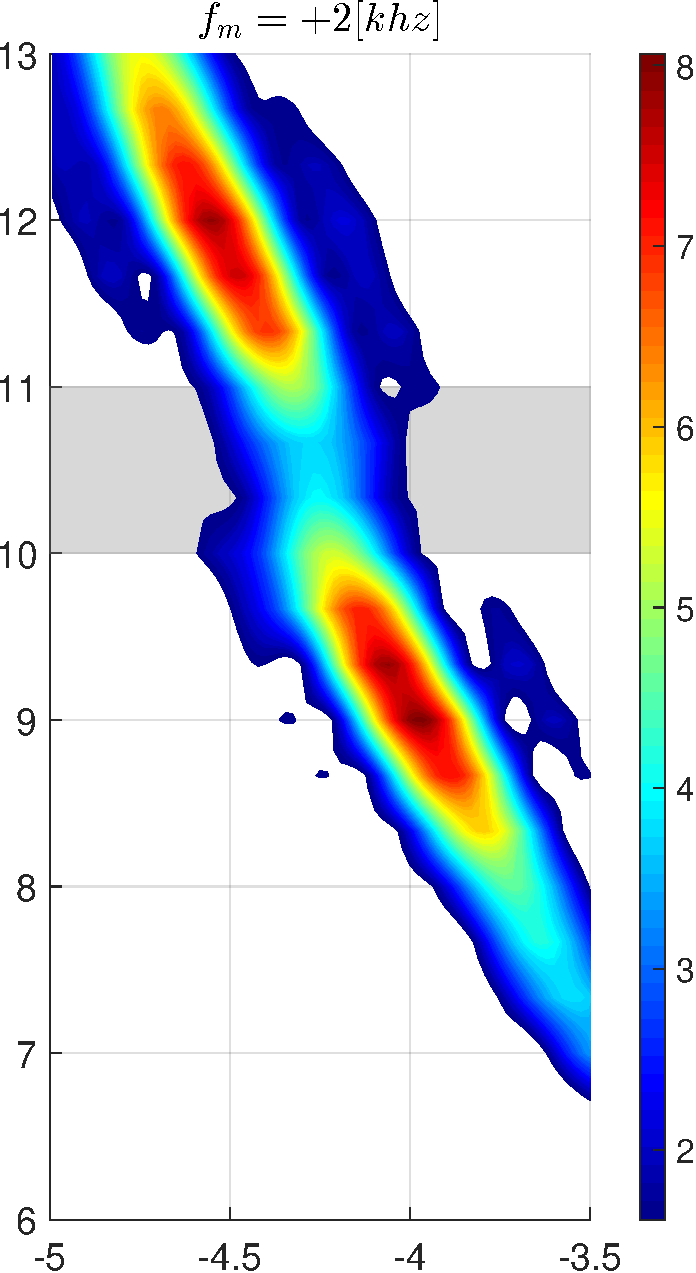
\includegraphics[width=0.3\textwidth]{img/MATLAB/EXP_nonreciprocal_@+2kHz.pdf}
    \hspace{2cm}
    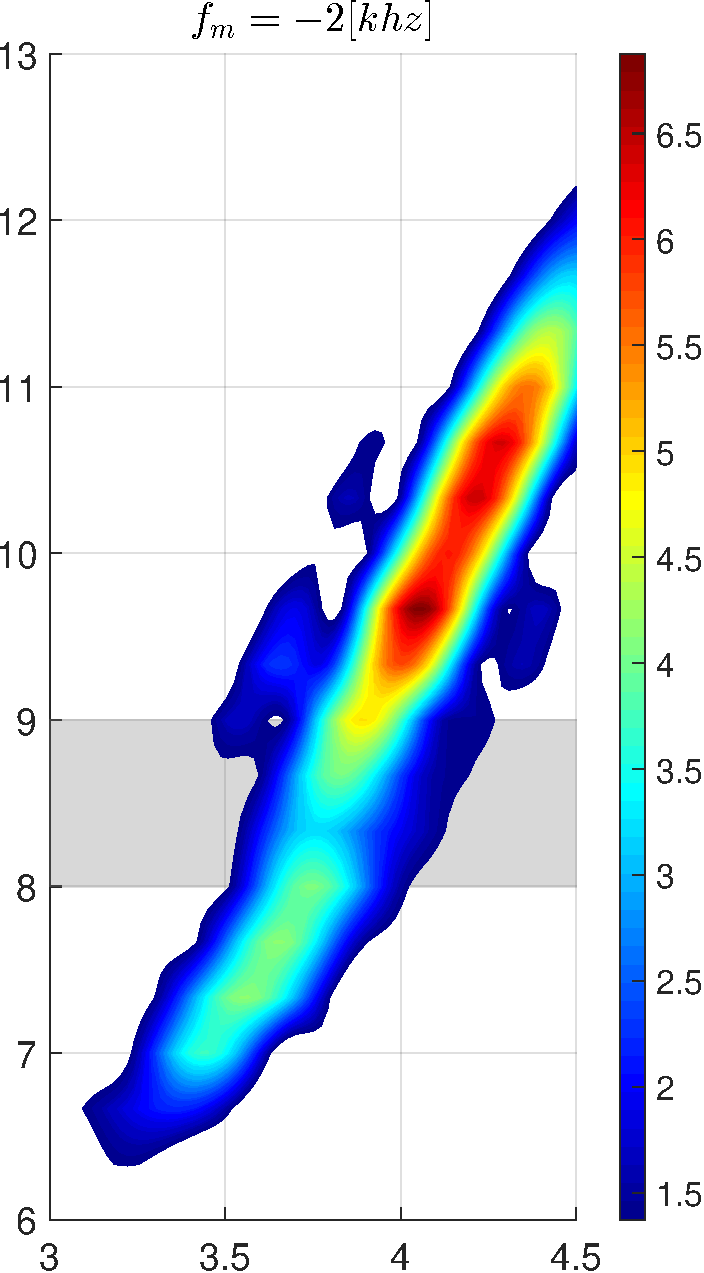
\includegraphics[width=0.3\textwidth]{img/MATLAB/EXP_nonreciprocal_@-2kHz.pdf}
    \caption{Dispersion diagram for the case of modulation frequency $f_m = \pm 2 kHz$.}
    \label{fig:nonreciprocal_behavior_2kHz}
\end{figure}

Two tests are now performed.

At first, a tone-burst excitation signal with central frequency $f_e = 8.4 kHz$ and delta frequency $\Delta f = 0.4 kHz$ is applied while modulating the shunts in one case at $f_m = +2 kHz$ and in the other case at $f_m = -2 kHz$.

Secondly, in a similar fashion, the higher frequency directional band-gaps is excited with a tone-burst signal having central frequency $f_e = 10.5 kHz$ and $\Delta f = 0.5 kHz$.
The shunts are modulated at the same frequencies as before ($f_m = \pm 2 kHz$).

The excitation signal is still applied as before at the same point along the beam, but the change in the sign of modulation frequency of the shunts has the same effect as changing the direction of the wave propagation.
Thanks to this property, the experimental setup remains unchanged while still allowing to investigate the nonreciprocal behavior of the structure.



\subsection{Results}
\label{subsec:nonreciprocal_behavior_results}

The obtained experimental data align with what has already been in present in Section \ref{subsec:space_time_modulation}: because of time-modualtion of the shunts and so of the piezoelectric patches, the structure responds differently to the same excitation signal depending on the direction of the travelling wave.

This aspect is visible also from the waterfall plots of the beam displacement.
The diagrams below shows the trasversal displacement of some points along the beam as a function of time.
Depeneding on the excitation signal and the modulation frequency, the displacement at the end of the beam is different in the two cases.

\paragraph{Lower directional band-gaps $f_{BG}^+ = [8, 9] kHz$}

The waterfall plots in Figure \ref{fig:nonreciprocal_behavior_8p4kHz} show the trasversal beam displacement for the case of excitation at $f_e = 8.4 kHz$ and modulation at $f_m = \pm 2 kHz$.

\begin{figure}[H]
    \centering
    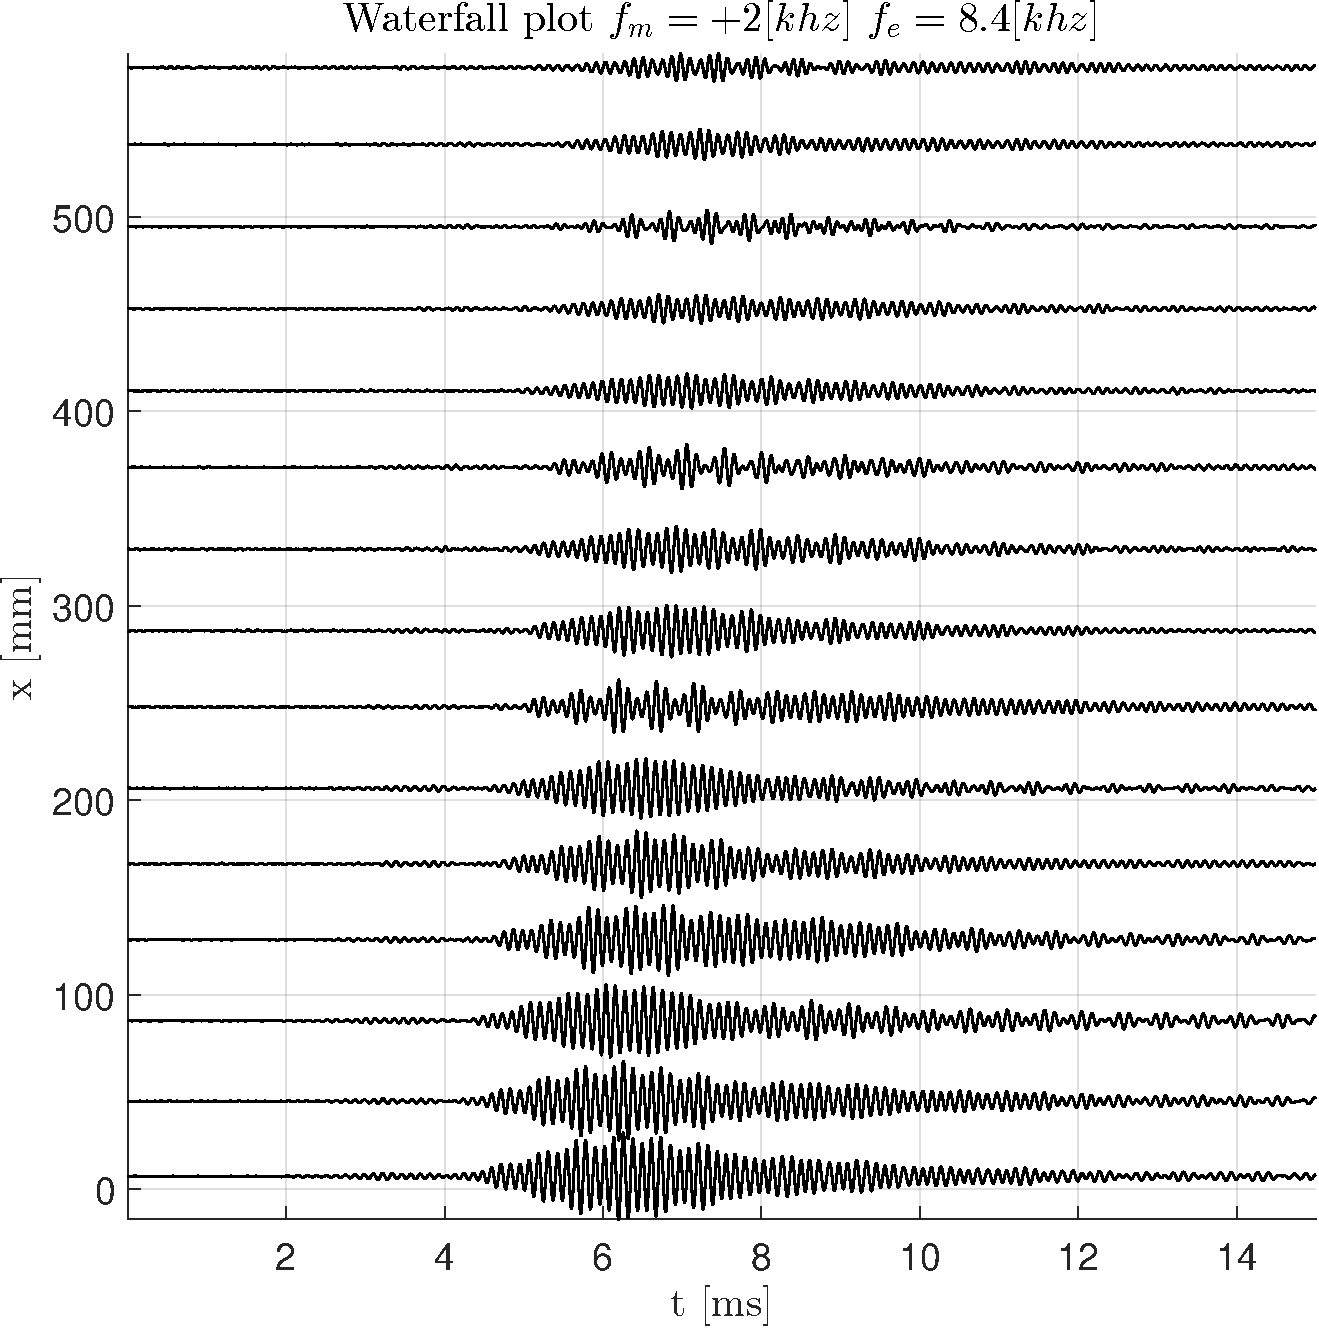
\includegraphics[width=0.45\textwidth]{img/MATLAB/EXP_Scan_time_narrow8p4kHz_2000plus.unv.pdf}
    \hspace{1cm}
    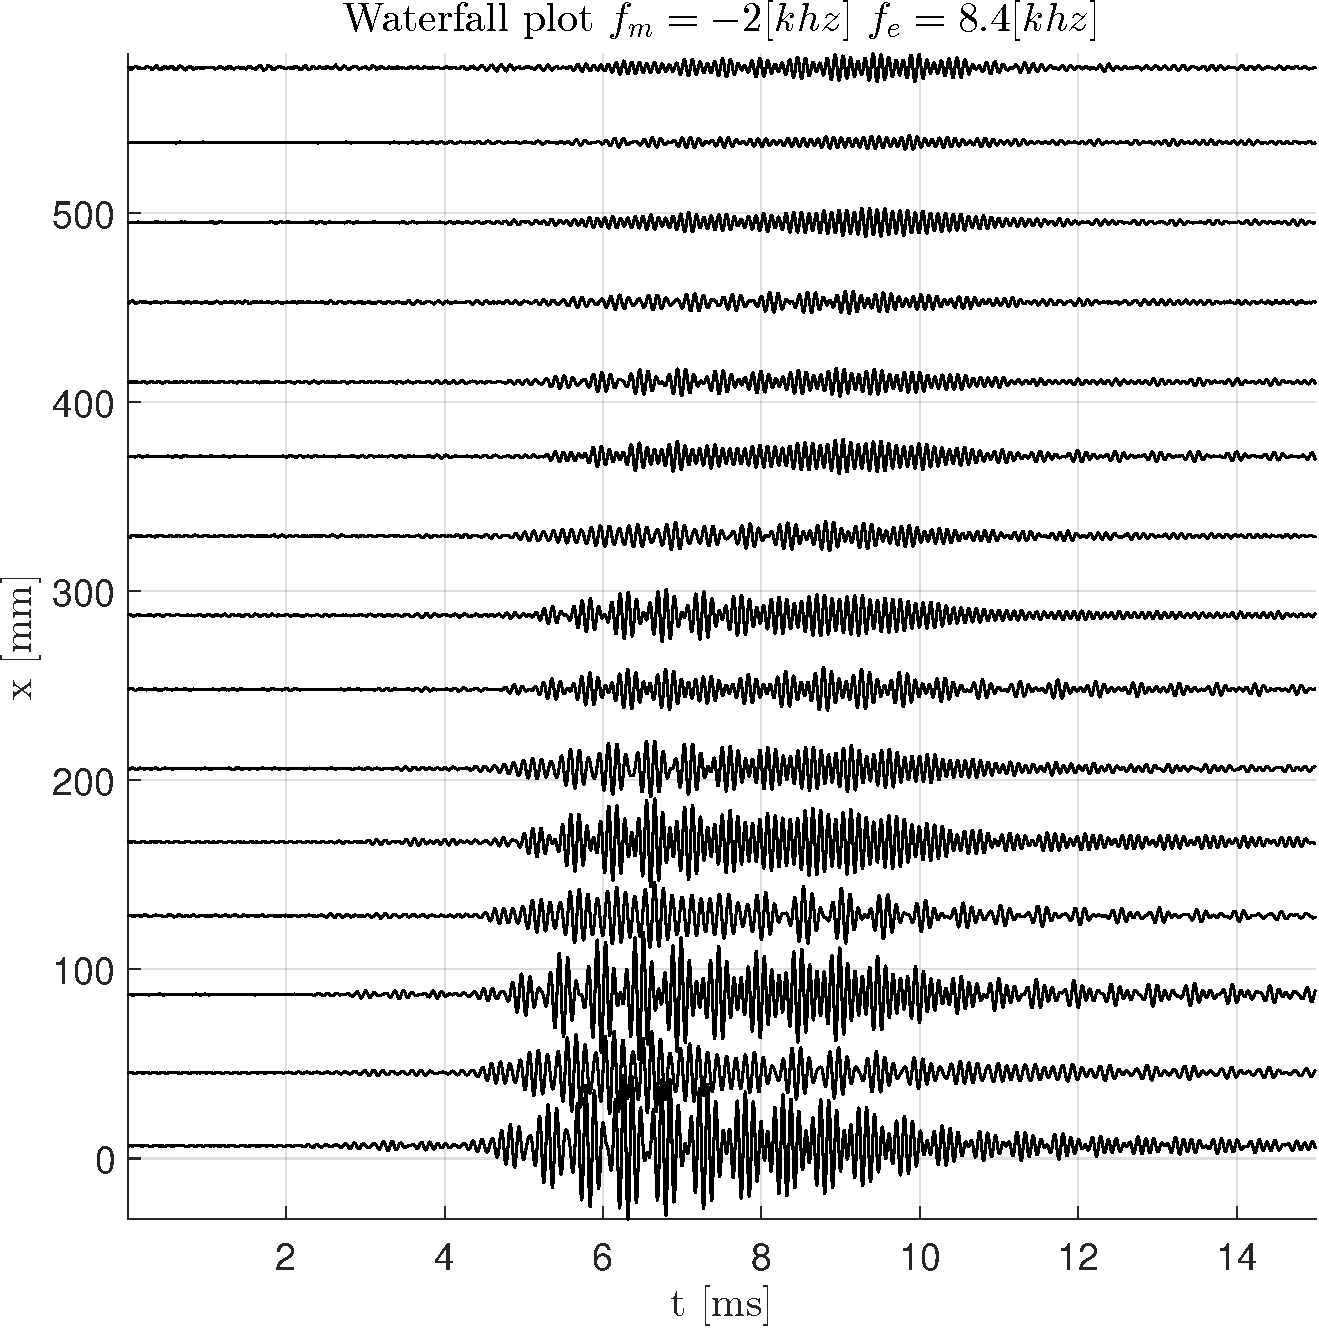
\includegraphics[width=0.45\textwidth]{img/MATLAB/EXP_Scan_time_narrow8p4kHz_2000minus.unv.pdf}
    \caption{Waterfall plot of the beam displacement for the case excitation at $f_e = 8.4 kHz$ and modulation at $f_m = +2 kHz$ (left) and $f_m = -2 kHz$ (right).}
    \label{fig:nonreciprocal_behavior_8p4kHz}
\end{figure}

Even if not clearly visible from the waterfall plots, the attenuation of the wave is different depending on the propagation direction.
Referring to Figure \ref{fig:nonreciprocal_behavior_2kHz}, we expected to obtain a stronger attenuation for the case of negative modulation frequency and, instead, a weaker attenuation for the case of positive modulation frequency.

Even if waterfall plots in this case do not show a clear difference in the attenuation of the wave, we can plot the spectra of the displacement signals at the end of the beam in the two cases to better observe the behavior of the structure.
The spectra are shown in Figure \ref{fig:nonreciprocal_behavior_8p4kHz_spectra}.

\begin{figure}[H]
    \centering
    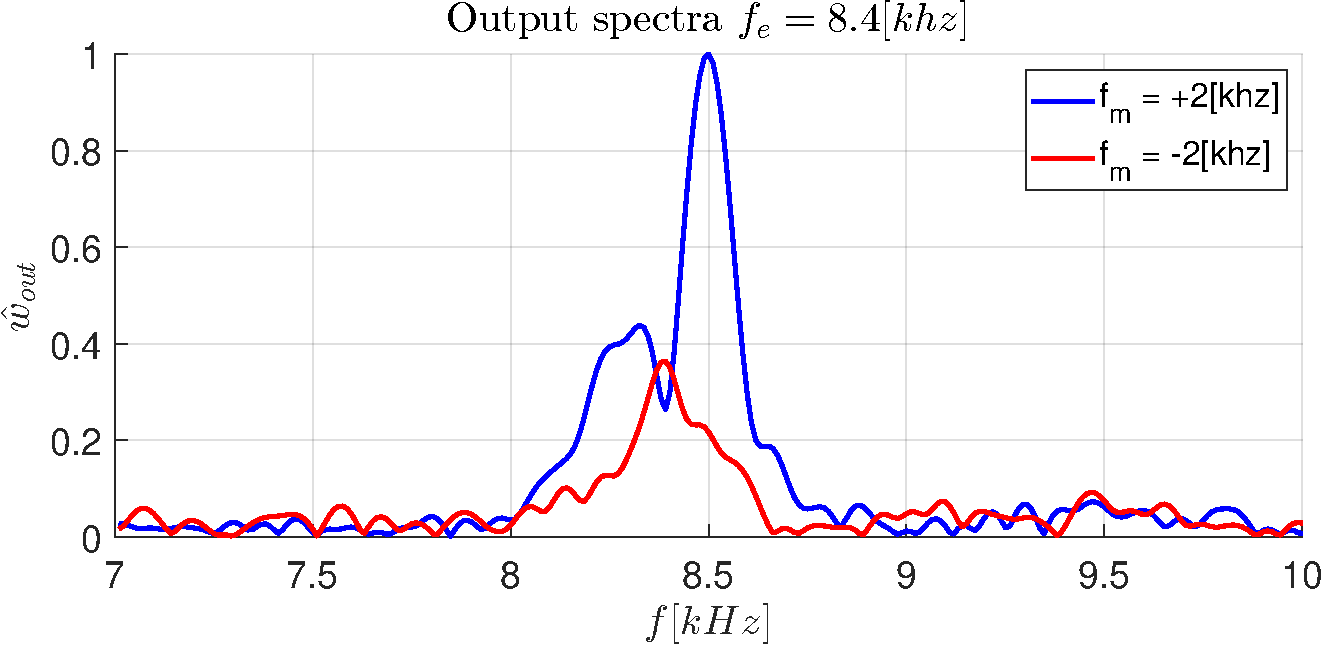
\includegraphics[width=0.7\textwidth]{img/MATLAB/Spectra_narrow8p4kHz_2000.pdf}
    \caption{Normalized spectra of the beam displacement at the end of the beam for the case of excitation at $f_e = 8.4 kHz$ and modulation at $f_m = \pm 2 kHz$.}
    \label{fig:nonreciprocal_behavior_8p4kHz_spectra}
\end{figure}

The spectra show that the attenuation of the wave is indeed different in the two cases.
The attenuation is in fact stronger in the case of negative modulation frequency, given that we find the directional band-gap at $f_{BG}^+ = [8, 9] kHz$.
On the other hand, the attenuation is weaker in the case of positive modulation frequency, given that no band-gap is present.


\paragraph{Higher directional band-gaps $f_{BG}^- = [10, 11] kHz$}

The waterfall plots in Figure \ref{fig:nonreciprocal_behavior_10p5kHz} show the beam displacement for the case of excitation at $f_e = 10.5 kHz$ and modulation at $f_m = \pm 2 kHz$.

\begin{figure}[H]
    \centering
    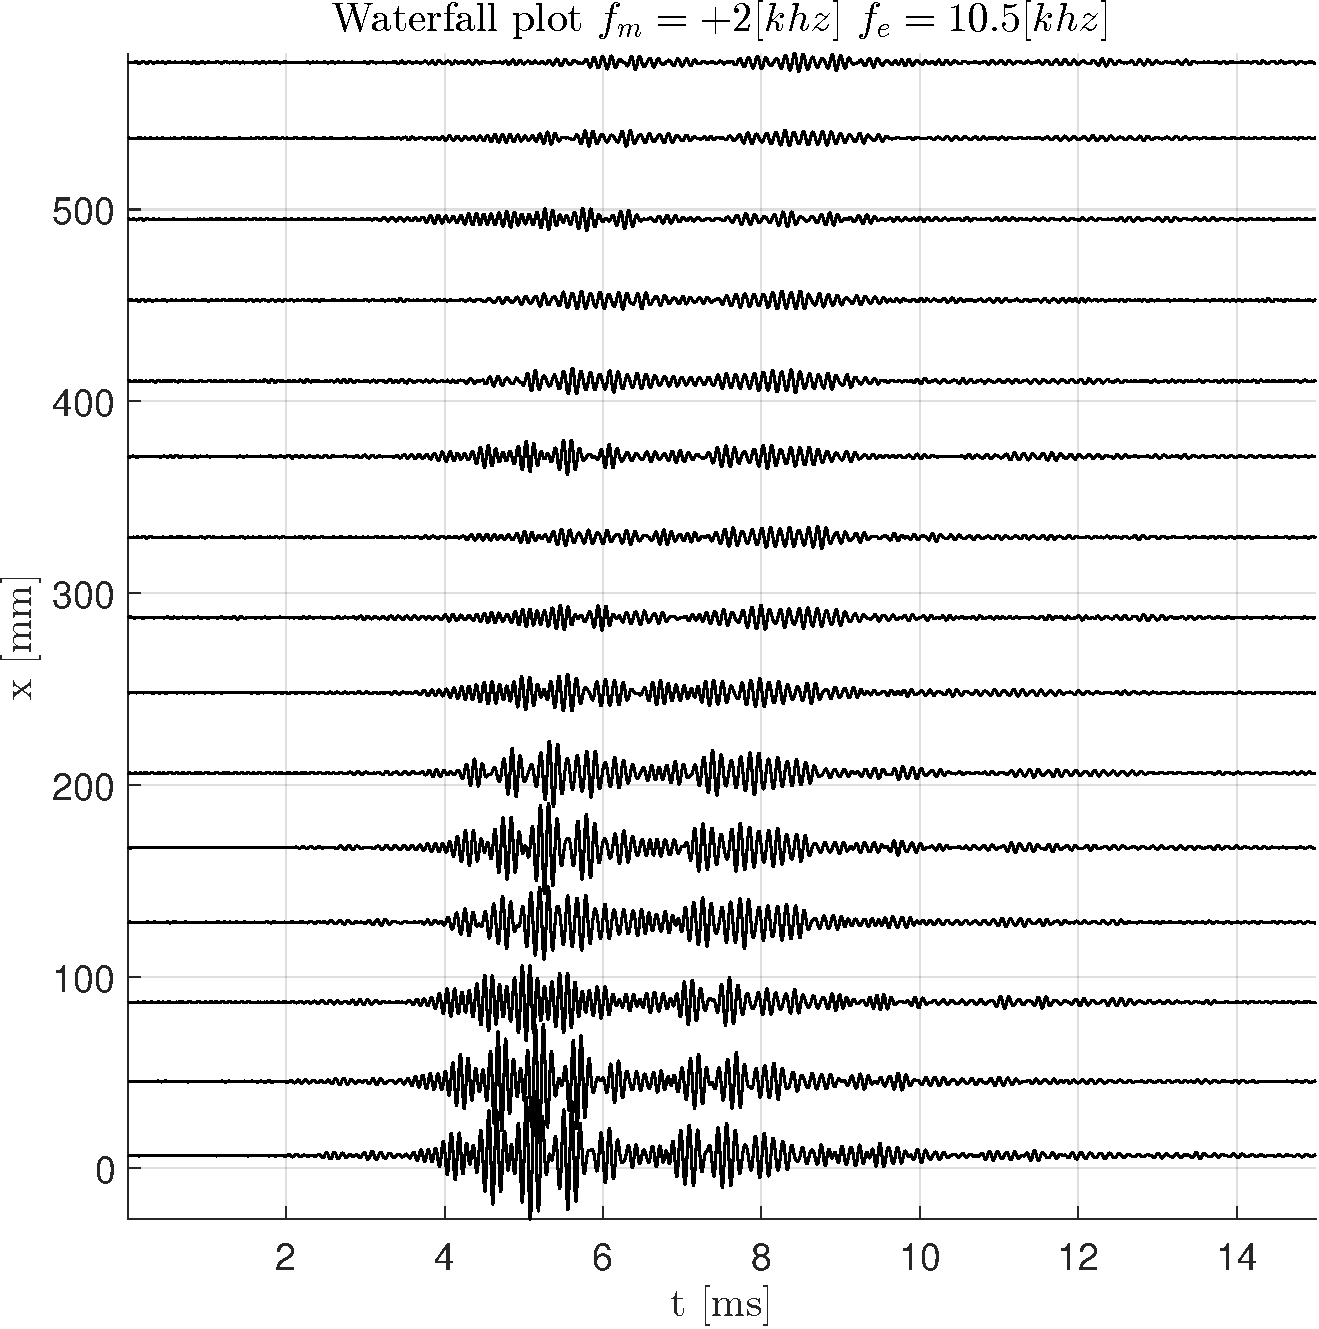
\includegraphics[width=0.45\textwidth]{img/MATLAB/EXP_Scan_time_narrow10p5kHz_2000plus.unv.pdf}
    \hspace{1cm}
    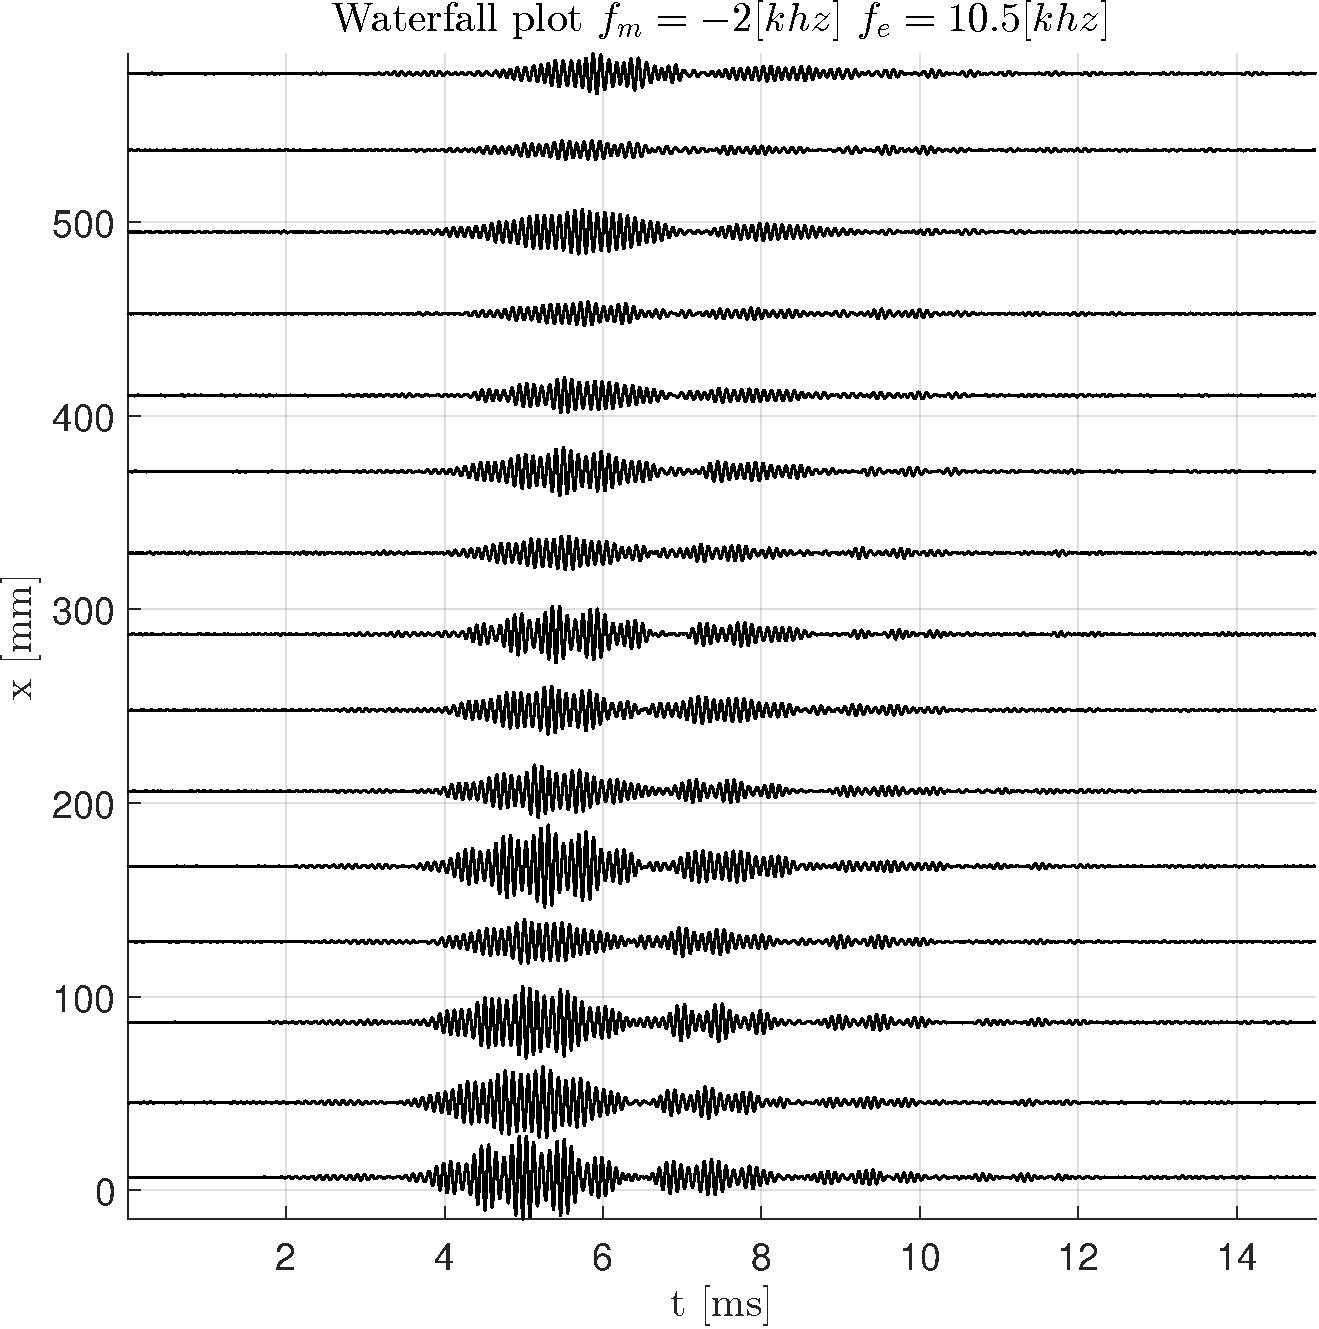
\includegraphics[width=0.45\textwidth]{img/MATLAB/EXP_Scan_time_narrow10p5kHz_2000minus.unv.pdf}
    \caption{Waterfall plot of the beam displacement for the case excitation at $f_e = 10.5 kHz$ and modulation at $f_m = +2 kHz$ (left) and $f_m = -2 kHz$ (right).}
    \label{fig:nonreciprocal_behavior_10p5kHz}
\end{figure}

The waterfall plots show a clear difference in the attenuation of the wave in the two cases.
Referring to Figure \ref{fig:nonreciprocal_behavior_2kHz}, we expected to obtain a stronger attenuation for the case of negative modulation frequency, and instead a weaker attenuation for the case of positive modulation frequency.
Figure \ref{fig:nonreciprocal_behavior_10p5kHz} confirms this expectation, showing a full band-pass behavior in one case and a full band-stop behavior in the other case.

The spectra of the beam displacement at the end of the beam are shown in Figure \ref{fig:nonreciprocal_behavior_10p5kHz_spectra}.

\begin{figure}[H]
    \centering
    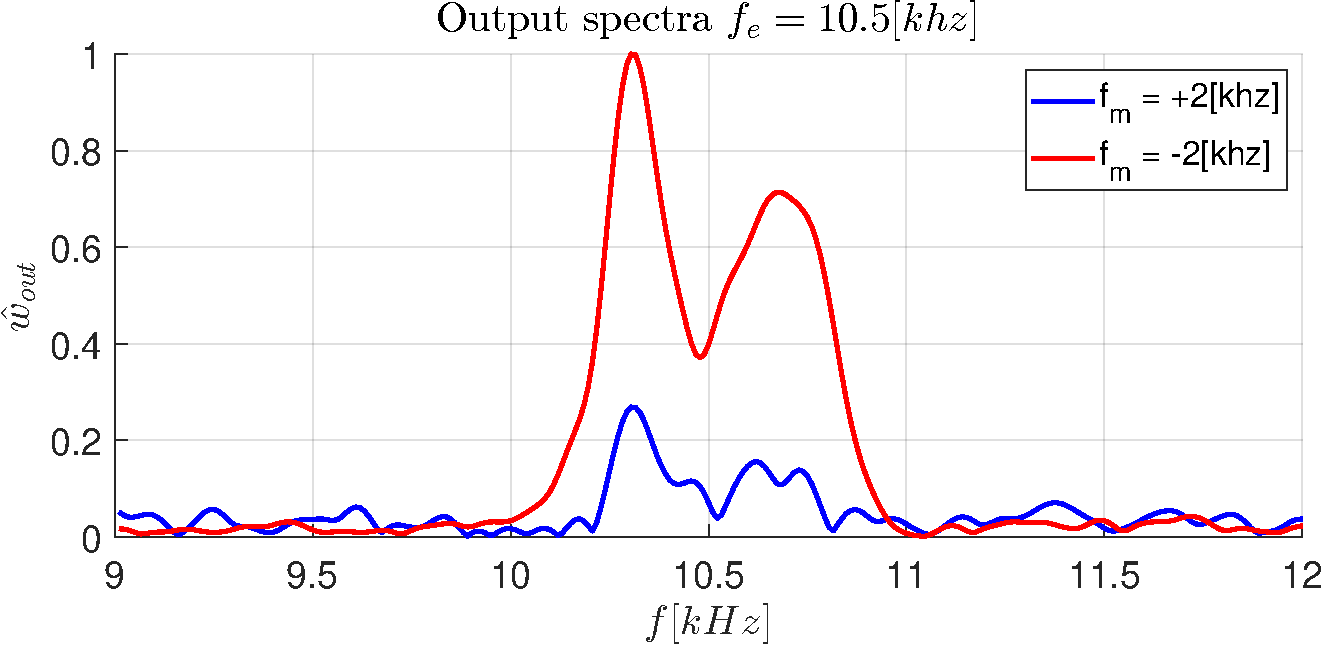
\includegraphics[width=0.7\textwidth]{img/MATLAB/Spectra_narrow10p5kHz_2000.pdf}
    \caption{Spectra of the beam displacement at the end of the beam for the case of excitation at $f_e = 10.5 kHz$ and modulation at $f_m = \pm 2 kHz$.}
    \label{fig:nonreciprocal_behavior_10p5kHz_spectra}
\end{figure}

Also the spectra analysis confirms the expected behavior.


